\documentclass[tikz, border=15pt]{standalone}
\usepackage{amsmath, amssymb,ctex}
\usetikzlibrary{arrows.meta}

\begin{document}
	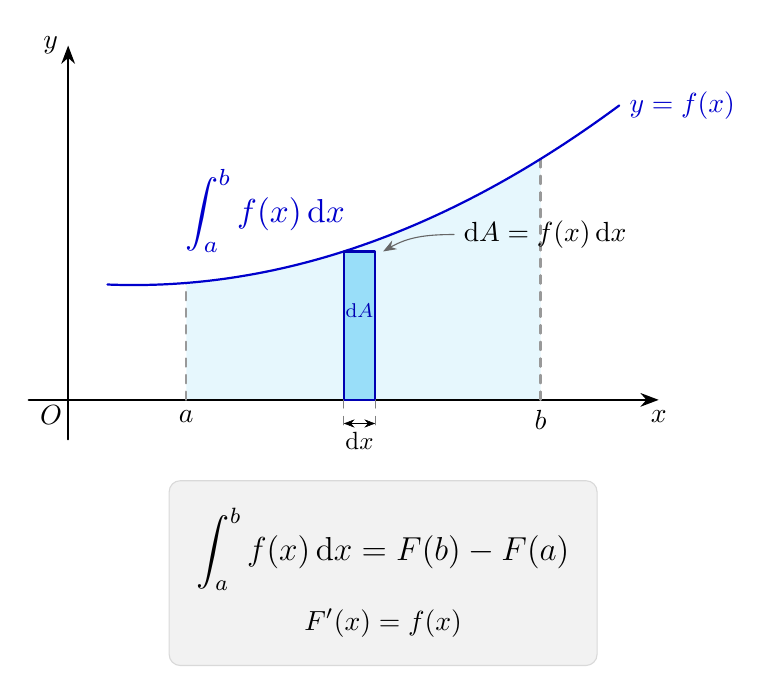
\begin{tikzpicture}[>=Stealth, line cap=round, line join=round]
		
		% ================= 1. 参数定义 =================
		\def\xmax{7.5}
		\def\ymax{4.5}
		
		\def\a{1.5}   % 积分下限
		\def\b{6.0}   % 积分上限
		
		% 定义一个平滑的函数 f(x)
		% f(x) = 0.06 * x^2 - 0.1 * x + 1.5
		\def\fx{0.06*\x*\x - 0.1*\x + 1.5}
		
		% ================= 2. 填充积分区域 =================
		% 绘制积分面积的整体浅色填充
		\fill[cyan!10] (\a, 0) -- plot[domain=\a:\b, samples=100] (\x, {\fx}) -- (\b, 0) -- cycle;
		
		% ================= 3. 绘制参考系与边界 =================
		% x 轴和 y 轴
		\draw[->, thick] (-0.5, 0) -- (\xmax, 0) node[below] {$x$};
		\draw[->, thick] (0, -0.5) -- (0, \ymax) node[left] {$y$};
		\node[below left, inner sep=2pt] at (0,0) {$O$};
		
		% 积分边界虚线
		\draw[dashed, thick, gray!80] (\a, 0) node[below, text=black] {$a$} -- (\a, {0.06*\a*\a - 0.1*\a + 1.5});
		\draw[dashed, thick, gray!80] (\b, 0) node[below, text=black] {$b$} -- (\b, {0.06*\b*\b - 0.1*\b + 1.5});
		
		% ================= 4. 绘制函数曲线 =================
		\draw[thick, blue!80!black, domain=0.5:7.0, samples=100] plot (\x, {\fx}) node[right] {$y = f(x)$};
		
		% ================= 5. 绘制微分面积元 (黎曼和微元) =================
		\def\xi{3.5}            % 微元位置
		\def\dx{0.4}            % 微元宽度 dx
		\def\fxi{0.06*\xi*\xi - 0.1*\xi + 1.5} % 微元高度 f(x)
		
		% 高亮显示单个矩形微元
		\fill[cyan!40, draw=blue!70!black, thick] (\xi, 0) rectangle (\xi+\dx, \fxi);
		
		% 标注微元宽度 dx
		\draw[<->, very thin] (\xi, -0.3) -- (\xi+\dx, -0.3) node[midway, below, scale=0.9] {$\mathrm{d}x$};
		\draw[dashed, thin, gray] (\xi, 0) -- (\xi, -0.4);
		\draw[dashed, thin, gray] (\xi+\dx, 0) -- (\xi+\dx, -0.4);
		
		% 标注微元面积 dA
		\node[text=blue!70!black, scale=0.9] at (\xi + \dx/2, \fxi/2) {{\footnotesize $\mathrm{d}A$}};
		
		% ================= 6. 添加数学说明文本 =================
		% 面积说明
		\node[scale=1.2, text=blue!80!black] at (2.5, 2.4) {$\displaystyle\int_a^b f(x) \, \mathrm{d}x$};
		
		% 曲线下方微元高亮说明
		\draw[->, thin, gray!80!black] (4.9, 2.1) node[right, text=black] {$\displaystyle\mathrm{d}A = f(x)\,\mathrm{d}x$} to[out=180, in=30] (\xi+\dx/2+0.3, \fxi);
		
		% ================= 7. 底部公式框 (牛顿-莱布尼兹公式) =================
		\node[fill=gray!10, rounded corners, inner sep=10pt, align=center, draw=gray!30] at (4, -2.2) {
			\large $\displaystyle\int_a^b f(x) \, \mathrm{d}x = F(b) - F(a)$ \\[2mm]
			\normalsize $\displaystyle F'(x) = f(x)$
		};
		
	\end{tikzpicture}
\end{document}